\section{Interaction Engineering - Fragenkatalog}
\subsection{Introduction}
\begin{enumerate}
	\item Erkläre Stärken und Schwächen des Menschens und des Computers in der Human-Computer Interaction!
	\begin{table}[!h]
		\centering
		\begin{tabular}{|p{20em}|p{20em}|}
			\hline
			Mensch & Computer\\
			\hline
			\tabitem Kreativität & \tabitem 'exakte'\footnote{Denke an max. Genauigkeit von Fließkommazahlen!} Berechnungen\\
			\tabitem Abstrahieren und Erzeugen von Modellen & \tabitem stundenlanges Ausführen derselben Aufgabe ohne zu Ermüden\\
			\tabitem auf Unerwartetes reagieren& \tabitem exakter Speicher (Gedächtnis)\\
			\hline
		\end{tabular}
		\caption{Stärken des Menschen und Computers in HCI. (Särken = Schwächen des anderen!)}
		\label{strength_of_hc}
	\end{table}
	
	\item Kernunterschied bei der Entwicklung von computional solutions und interactive solutions
	\begin{itemize}
		\item Interaction: Kernfaktor ist das Human Computer Interface
		\item Computational: Kern ist effizienter Algorithmus(?)
		\item Rechenleistung steigt immer weiter während menschliche Aufnahmefähigkeit stagniert/konstant ist
		\item Kernfaktor bei der Informationsverarbeitung durch den Menschen ist das Interface
		\item $\Rightarrow$ Interaction soll smooth und effizient; Feedback soll reich an Informationen und instantan sein
		\item HC-Interaction - Mensch und Computer gehen Hand in Hand, jeder erfüllt die Aufgaben, die er am besten lösen kann (siehe Tabelle \ref{strength_of_hc})
		\begin{table}[!h]
			\centering
			\begin{tabular}{|l|l|}
				\hline
				\textbf{Computation} - closed system & \textbf{Interaction} - open system\\
				\hline
				\tabitem Eingabe & \tabitem Veränderung in der Umwelt\\
				\tabitem Verarbeitung & \tabitem Empfange Events\\
				\tabitem Ausgabe  & \tabitem Reagiere auf Events\\
				\tabitem deterministisch, Endzustand & \tabitem endlos, nichtdeterministisch\\
				\hline
			\end{tabular}
		\end{table}
	\end{itemize}
	
	\item Action Cycle by Norman
	\begin{enumerate}
		\item Mensch hat Ziel im Kopf (Goal)
		\item Planen der notwendigen Schritte (Plan)
		\item Spezifizieren der Schritte (Specify) 
		\item Umsetzen der Schritte in der Welt (Perform)
		\item Feedback in der Welt beobachten (Perceive) 
		\item Feedback interpretieren (Interpret)
		\item Ergebnis mit Zielen vergleichen (Compare)
		\item Beginne bei Schritt 1 bzw. 2
	\end{enumerate}
	\begin{figure}[!h]
		\centering
		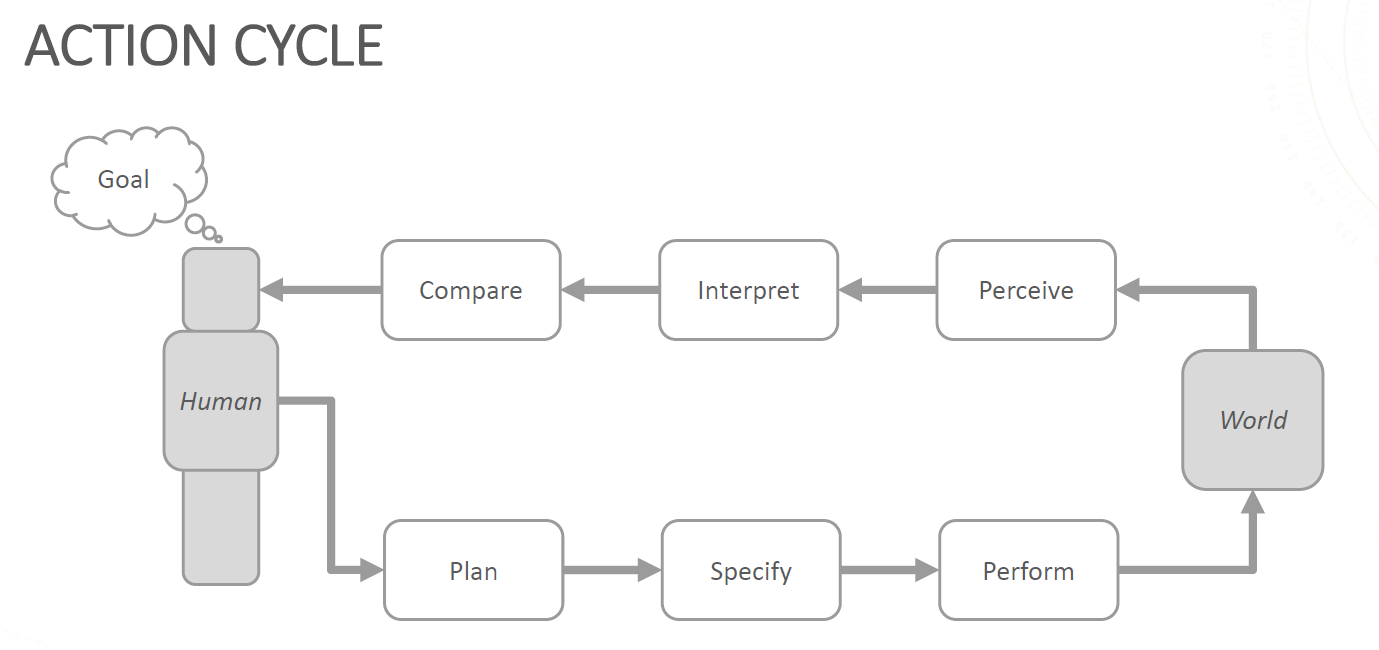
\includegraphics[scale=0.4]{img/action_cycle.png}
		\caption{Action Cylce nach Norman}
	\end{figure}
	
	\item Iteration/Bsp für den Action Cycle\\
	Am Beispiel: Kaffee holen in der Mensa
	\begin{itemize}
		\item \textbf{Goal:} Kaffee in der Mensa holen
		\item \textbf{Plan:} Aus dem Büro gehen
		\item \textbf{Specify:} Operation - Türgriff betätigen um Bürotür zu öffnen
		\item \textbf{Perform:} Türgriff drücken
		\item \textbf{Perceive:} Griff öffnet das Schloss, Tür öffnet sich
		\item \textbf{Interpret:} Tür ist offen
		\item \textbf{Compare:} Schritt erfolgreich, Führe weitere Schritte aus
	\end{itemize}
	
	
	\item  Gulf of Execution and Evalutation
	\begin{itemize}
		\item \textbf{Execution}\\
		beschreibt die Mühe/Aufwand der angestrebten Aufgaben\\
		Kann ich das tun? Wo ist die notwendige Funktionalität? Welches Gerät nutze ich? Wie führe ich das Kommando aus?
		\item \textbf{Evaluation}\\
		Beschreibt die Mühe/Aufwand die Veränderung der Umwelt zu interpretieren\\
		Ist überhaupt etwas passiert? Wo ist etwas passiert? Was ist passiert? Passen Effekt und Absicht zusammen?
		\item Interaction cost = Summe des physischen und mentalen Aufwandes um ein Ziel zu erreichen
		\item Beispielhaft am Action Cycle:
		\begin{itemize}
			\item Cost of Decision (Goal): Fokus muss auf Teilmenge von Informationen und Interfaces gelenkt werden
			\item Cost of System Power (Plan): Übersetzen von Zielen im Kopf in Operationssequenzen ist schwer, insbesondere für komplexe Systeme
			\item Cost of visual clutter/visuelle Überfuütung/reizung (Perceive): Bsp - Mouse Hover Effekte erzeugen Überreizung und erschweren Zustandswahrnehmung 
		\end{itemize}
	\end{itemize}
	
	\item The Three levels of interaction
	\begin{itemize}
		\item \textbf{low level:} Selection and Manipulation
		\item \textbf{inter-mediate level:} Exploration and Navigation
		\item \textbf{high level:} Problem-solving
	\end{itemize}
	
	\item The levels of (human) interaction processing
	\begin{itemize}
		\item Instinktiv (Perform and Perceive): vollkommen unterbewusst, ohne Kontrolle, schnell, Basisfähigkeiten - Bsp: Arm bewegen um Türgriff zu fassen
		\item Behavioral (Specify and Interpret): teilweise unterbewusst, leichte Kontrolle, schnell, gelernte Fähigkeiten - Bsp: Drücken der Klinke öffnet Tür
		\item Reflective (Plan and Compare): volles Bewusstsein, langsam, komplexe Analyse - Bsp: Tür ist offen, was bedeutet das?
	\end{itemize}
	
	\item at least 5 golden rules or guidelines for interaction\\
	\textbf{Golden Rules - Norman}
	\begin{enumerate}
		\item Discoverability: Welche (möglichen) Aktionen können bestimmt werden?
		\item Feedback: reichhaltiger und kontinuierlicher Fluss an Informationen über den Zustand
		\item Affordances: angemessene Aufforderungen um die gewünschte Aktion durchzuführen
		\item Signifiers: effiziente Signalgeber für Discoverability und Feedback
		\item Mappings: gute Zuordnung zwischen Controls and Actions
	\end{enumerate}
	\textbf{Guidelines - Shneiderman}
	\begin{enumerate}
		\item Konsistenz: ähnliche Situationen sollen ähnliche Aktionen erfordern
		\item Universal Usability: Assistenz anbieten (Hilfe, Shortcuts,..)
		\item Informative Feedback: Feedback für jede Useraktion
		\item Closure: klarer Beginn, Ablauf und Ende einer Aktion; kombiniere mit Punkt 3
		\item Prevent Error: vermeide fehlerhaften input, Recover from user error
		\item Easy reversal of actions: zb undo redo
		\item internal locus of control: User kontrolliert das System
		\item reduce short-term memory load: keep it simple
	\end{enumerate}
\end{enumerate}

\textbf{Sonstige Notizen}
\begin{itemize}
	\item Vor- und Nachteile der Interaction
	\begin{table}[!h]
		\centering
		\begin{tabular}{|p{20em}|p{20em}|}
			\hline
			\textbf{Vorteile} & \textbf{Nachteile}\\
			\hline
			\tabitem ist mächtiger als ''Algorithmen'' & \tabitem User muss wissen \textit{was} er/sie möchte\\
			\tabitem anspruchsvolleres Verhalten & \tabitem User muss wissen \textit{wie} er/sie den Computer bedienen muss um das Ziel zu erreichen\\
			 & \tabitem Anwendung ist zustandsbehaftet -> User kann sich verlieren/steckenbleiben (stateful things can be broken)\\
			\hline
		\end{tabular}
	\end{table}
	
	\item Bottlenecks - Processing: CPU, RAM, Netzwerk etc.. mittlerweile in vielen Anwendungsgebieten nicht mehr so relevant
	\item Bottlenecks - Information: enorm wichtig welche Daten auf dem kleinen Bildschirm am Ende angezeigt werden (viele, viele Daten gespeichert; welche Davon sind wichtig und werden angezeigt?)
	\item Bottlenecks - Aufnahmefähigkeit Mensch
\end{itemize}


\subsection{Basics of Graphics and Interaction Programming}
\begin{enumerate}
	\item Illustrate the interplay of the action cycle and the model-view-controller pattern!
	\begin{figure}[!h]
		\centering
		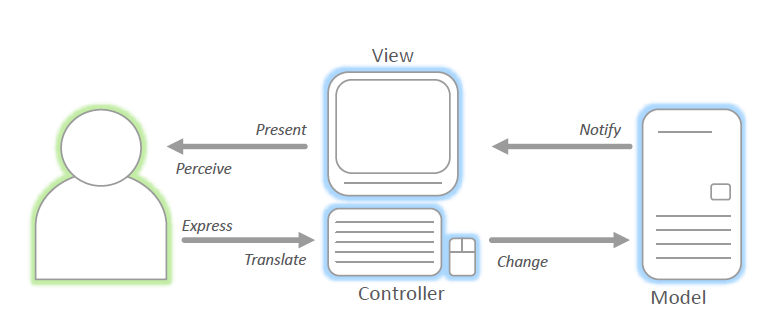
\includegraphics[scale=0.5]{img/ac_with_mvc.png}
		\caption{Zusammenspiel Action Cycle und MVC}
	\end{figure}
	
	\item Discuss different forms of presentation!\\
	Wahrnehmungen durch die 5 Sinne, geordnet nach Relevanz für HCI:\\
	Visuell, Audio, Fühlbar, Geruch, Geschmack\\
	wichtige Aspekte: Bandbreite, Aufmerksamkeit, Vergänglichkeit/Flüchtigkeit
	
	\item Discuss different forms of expression!\\
	Sprache, Point \& Gestures, Physical movement (sich selbst, Objekte wie Maus, Tastatur..)\\
	wichtige Aspekte: Genauigkeit, Geschwindigkeit, Aufwand
	
	\item Discuss pros and cons of uni-modal and multi-modal interaction!\\
	\textbf{Uni-Modal:} genau eine Form der Presentation und Expression (zb Visuell und Point \& Gestures) $\Rightarrow$ ein Kanal\\
	\textbf{Multi-Modal:} mehrere Formen/Kanäle; zb Visuell, Audio und Touch, Sprache, Point..
	\begin{table}[!h]
		\centering
		\begin{tabular}{|l|p{15em}|p{15em}|}
			\hline
			&	\textbf{Vorteile} & \textbf{Nachteile}\\
			\hline
			Uni-Modal & einfache Implementierung & nur ein Kanal\\
			\hline
			Multi-Modal & umfangreiche Formen der Interaktion & komplexe Implementierung und schwieriger zu lernen (für den User)\\
			\hline
		\end{tabular}
	\end{table}
	
	\item What are the mental, implementation and represented model? Why are they important?
	\begin{itemize}
		\item \textbf{Mental:} gedankliche Vorstellung des Modells; entspricht menschlicher Natur; beschreibt v.a. Operationen zum Erreichen des Ziels
		\item \textbf{Implementation:} interne Darstellung; technisch limitiert und vom Entwickler vorgegeben; enthält Daten, Parameter, Algorithmen,...
		\item \textbf{Represented:} Darstellung des (Implementation) Models auf dem PC; vom Entwickler vorgegeben;
	\end{itemize}
	
	\begin{figure}[!h]
		\centering
		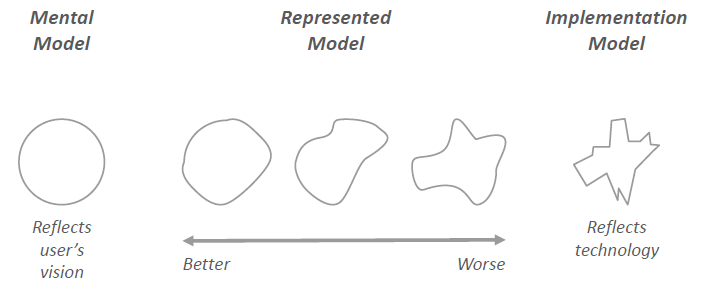
\includegraphics[scale=0.5]{img/models.png}
		\caption{Zusammenspiel der 3 Modelle}
	\end{figure}
	\textit{Important}, weil Mental Model nicht 1:1 in Computer dargestellt werden kann; müssen abstrahieren
	
	\item What is a graphics context and what can it be used for?\\
	Wird gestellt vom Window System und ist verknüpft mit dem Zeichenareal.\\
	Stellt Funktionalitäten zum Zeichnen bereit.
	
	\item Explain the basic procedure for drawing paths!\\
	begin path; move to; add (line, curve, arc,..); end path
	
	\item Name three interaction devices and characterize the input they deliver\\
	Pointing Device (Maus): absolute oder relative Koordinaten\\
	Triggers (Tasten)\\
	Value Input (Sensoren)

	\item Give examples of atomic and composite inputs!\\
	atomic: single click, Bewegung des Zeigers, aktiviere Trigger,..\\
	composite: double click, drag n drop, Gesten,...
	
	\item Illustrate the interconnections between model, view and controller in MVC pattern!
	\begin{figure}[!h]
		\centering
		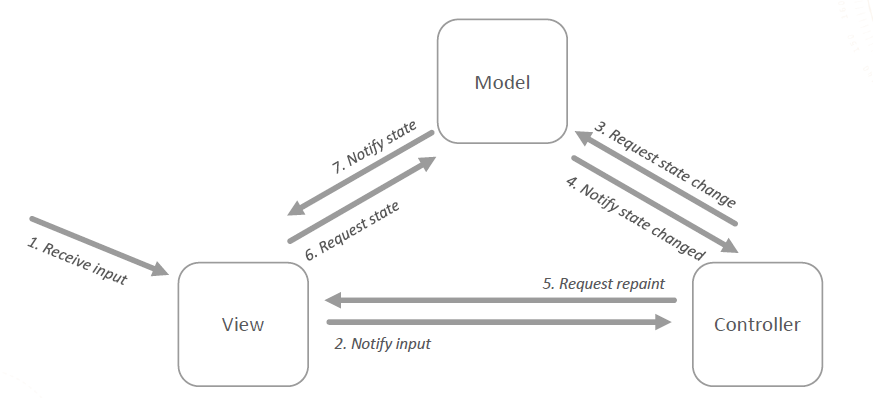
\includegraphics[scale=0.5]{img/mvc_interconnection.png}
		\caption{Interconnection der drei Bestandteile des MVC Pattern}
	\end{figure}
	
	\item Discuss advantages and disadvantes of the MVC!
	\begin{table}[!h]
		\centering
		\begin{tabular}{|p{20em}|p{20em}|}
			\hline
			\textbf{Vorteile} & \textbf{Nachteile}\\
			\hline
			klare konzeptuelle Trennung der Bestandteile & \tabitem enge Kopplung der Komponenten (durch Interaktion)\\
			\tabitem Entwurf für generelle Architektur & \tabitem komplex zu implementieren\\
			\hline
		\end{tabular}
	\end{table}
	
	\item What loop is the fundamental ingredient of interactive systems!\\
	\textbf{event loop:} Endlosschleife von Reaktionen auf Events; verschiedene Eventtypen; verschiedene Reaktionen
	
	\item Name at least five types of events in interaction systems!
	\begin{itemize}
		\item Application level: loaded, finished,..
		\item Widget level: Repaint, Resize, Activated, focused,...
		\item Input level: key pressed/released/typed,.. Touch start/moved/end, Mouse pressed/...
		\item Window System signals external event: repaint of window required; resize of window; Input von Peripherie (zb Maus)
		\item Application signals internal events: state change, timer elapsed
	\end{itemize}
	
	\item How are events propagated in interactive systems?\\
	Werden in EventQueue reingesteckte und nach FIFO verarbeitet;\\
	Dispatch Events: Traversiere Window Tree und wähle vorderstes Fensters aus\\
	Receive Events: definiere Verhalten bei Event; ausgeführt durch Listener
	
	\item How can callback functions be used to react to events?\\
	Callback als Parameter einer Funktion -> Funktion ausgeführt, dann führe Callback aus. Auf Events: Ich sage Programm mach etwas und du sollst mir Bescheid geben(=callback), Ausführung erzeugt Event und callback wird gerufen(omfg.. xD)\\
	gut für basic (device) events; but limited flexibility
	
	\item What are delegates and listeners?
	Interface um auf Events zu reagieren; Logik muss vom Entwickler umgesetzt werden\\
	cover many different events, also user-generated ones; but sometimes clomplex
	
	\item What are signals and slots and which toolkits make use of them?
	QT, GTK+,.. Kommunikation zwischen Objekten; Signal wird emitted wenn Event auftritt; Slot = Funktion die bei bestimmtem Event aufgerufen wird\\
	ähnlich zu Callbacks, aber mit höherer Flexibilität
	
	\item Express in pseudo code the main event loop and explain its components!\\
	Block and render -> wartet auf Event und rendert nur bei Bedarf neu
	\begin{lstlisting}
	while (true || event != QUIT) {
		event = wait_for_event();
		do_repaint = update_model(event)
		if (do_repaint) {
			render_model()
		}
	}
	\end{lstlisting}
	check and render full-throttle -> render mit jedem Durchlauf und reagiert nur auf Events
	\begin{lstlisting}
	while (true || event != QUIT) {
		if (check_for_event()) {
			event = get_event()
			update_model(event)
		}
		render_model()
	}
	\end{lstlisting}
		
	\item What is a disadvantage of method overriding for reacting to events?
	sollte in Sub-Class ausgelagert werden um Custom Verhalten umzusetzen; im Gegensatz zum Listener Konzept wesentlich unübersichtlicherer Code
\end{enumerate}


\subsection{Fundamental Interaction Concepts}
\begin{enumerate}
	\item At which three levels can interaction be considered?
	\begin{itemize}
		\item Low level: basic picking and manipulation\\
		Event Notifications: \textit{Etwas} ist passiert;\\
		Event Type: \textit{Was} ist passiert;\\
		Interaction abhängig vom räumlichen Kontext: also \textit{wo} etwas passiert ist;\\
		Interaction Handling = Event Notification + Event Type + räumlicher Kontext
		\item Intermediate level: Kombiniere low level Techniken zu navigieren, exploration, modellieren
		\item High level: kombiniere intermediate level Techniken zu komplexen Prozessen (Understanding, Kreativität)
	\end{itemize}
	
	\item Why is picking necessary for human-computer interaction?\\
	Picking - Grundelement für Interaktion, Mensch ist es in realer Umgebung gewohnt Dinge anzufassen bevor er mit ihnen interagiert\\
	Für Picking extra Ebene -> MDPC - model, display view, picking view, controller\\
	Picking view beschreibt Interaction Geometry (ermöglicht räumlichen Kontext) -> Regionen mit denen interagiert werden kann\\
	Vorteil der View Trennung: einfacheres Modellieren, Testen; GUI kann ausgetauscht werden ohne Interaktion zu verlieren; verbessertes Verhalten (Bsp: Dropdown Mouse Movement)
	
	\item Characterize the picking problem! What is given, what is sought(gesucht)?
	Given: Interaction Geometrie $G = \{g_1,\ldots, g_n\}$ und eine Position auf dem Bildschirm $P = (x,y)$\\
	Gesucht: Interaction Geometrie $G' \subset G$ am Punkt $P$, wobei\\
	$|G| = 0$, wenn nichts matcht\\
	$|G| = 1$, für einen eindeutigen Match\\
	$|G| > 1$, für mehrere Matches\\
	\textit{Technical Requirements:} Speed -> Picking muss innerhalb ms identifiziert werden; Picking requests können sehr schnell eintreffen\\
	Genauigkeit: muss exakt sein, front-most object\\	
	\textit{Human R:} Fitt's law: betrachte beim Design die Zeit, die Nutezr für Interaktion vor. benötigen wird
	
	\item Explain the role of "essential geometry" and "MDPC"!
	MPDC - siehe 2 Fragen vorher\\
	Essential Geometry - Grundlegende Geometrie (Punkte, Linien, Shapes, Objects, Rays):\\
	Controller muss drag region auf model mappen. Regions setzen sich zusammen aus den essential Geometrie Bestandteilen -> Essential Geometry dient quasi als Connection zw. View und Controller beim Picking\\
	Vier muss Regions kennen (zwecks rendern)
	
	\item Sketch the basic implementation strategies for picking!\\
	\textbf{Screen Space Picking}
	\begin{itemize}
		\item Render Szene in Picking Buffer, Geometrie hat dort eine ID
		\item Benutze Pointer Koordinaten als direkter Index für den Picking Buffer
		\item Javascript: Draw Path -> apply HitRegion -> Event: Abfrage welche HitRegion getroffen wurde
		\item OpenGL: zusätzliches RenderTarget -> Elementen IDs zuweisen -> Geometrie mit Hilfe der IDs (in Form von Farben) rendern -> look up ID from picking buffer
	\end{itemize}
	\textbf{Object Space Picking}
	\begin{itemize}
		\item Projiziere Pointer in die Szene mit Hilfe inverser Transformationen
		\item Berechne Containment/Intersection mit der Szenen Geometrie
		\item Nearest Neighbor Search:
		\item Finde Geometrie am nächsten zu $P$
		\item Optional: beschränke Picking auf Epsilonumgebung
		\item machbar für Punkte(0D) und Linien(1D)
		\item Punkte: Berechne Distanz von P zu allen Punkten; nimm Punkt mit geringster Distanz
		\item Linien: Lot von P auf Linien fällen -> nimm Linie mit kürzestem Lot\\
		\\
		\item Containment Search:
		\item Finde Geometrie, die P enthält
		\item machbar für Shapes (2D) und Objekte (3D)
		\item Shapes: Check if P is contained in geometry
		\item Objects: Wandle P in Ray/Strahl um und prüfe ob Strahl die Dreiecke des Objekts schneidet
	\end{itemize}
	
	\item Discuss different ideas to accelerate the picking!
	\textbf{Computation Performance}
	\begin{itemize}
		\item Reduziere Komplexität der Geometrieberechnung
		\item Sub-linear Search -> benutze hierarchische Strukturen (Bäume,..) um Suchen zu beschleunigen
		\item Pointer Kohärenz: gucke zunächst in Nachbarschaft
	\end{itemize}
	\textbf{User Performance}
	\begin{itemize}
		\item unterschiedliche Picking Mechanismen mit teils mehr Features
		\item Sticky Cursor
		\item Bubble Cursor
		\item Bubble Lens
	\end{itemize}
	
	\item Selektionsarten:
	\begin{itemize}
		\item Click Selection: Nutzer klickt Elemente einzeln an -> Serie von einzelnen Pickingaktionen; typisch: Simple Click, Strg+ Click, Shift + Click
		
		\item Rectangle Selection: Nutezr zeichnet Rechteck. Selektion entweder\\
		\textit{inside}: shape was auch immer muss zu 100\% im Rechteck enthalten sein\\
		gut für kleine, reguläre Elemente -> Bsp Desktop Icons\\
		Nachteil: bei unregelmäßigen oder großen Strukturen muss ich gut abschätzen können, ob mein Rechteck alle Elemente einkapselt
		\textit{overlap}: Elemente müssen Rechteck nur schneiden\\
		Vorteil: gut für unregelmäßige und große Elemente (zb Landkarte)\\
		Nachteil: Frage: wie viel muss geschnitten werden?!
		
		
		\item Lasso Selection: Selektion innerhalb free-form shape -> Nutzer zeichnet mit Maus quasi eine freie Form und innerhalb dieser wird selektiert
	\end{itemize}
	
	\item Discuss pros and cons of "inside" and "overlap" selection!
	siehe Frage vorher
	
	\item Grundlegend: Manipulation\\
	Object der Szene -> Interaktion benutzt um Geometrie und Eigenschaften des Objektes zu ändern\\
	View auf die Szene -> Kameramanipulation -> verändert die Perspektive auf die Szene\\
	\\
	Constrained Manipulation: Manipulation nur in bestimmten Bedingungen mgl, Bspw. Scrollbar nur in bestimmte Richtungen manipulierbar
	
	\item What is the difference between absolute and relative manipulation?
	Mappen des räumlichen Kontexts auf die Manipulation, entweder \\
	absolute: Punkt im Raum wählen -> dann Ergebnis -> abhängig von der aktuellen Pointer Position\\
	relativ: Pfad durch den Raum wählen -> dann Ergebnis -> Ergebnis abhängig von Serie von Pointer Positionen
	
	\item Wofür Navigation? -> große Mengen an Daten können nicht alle auf dem Bildschirm dargestellt werden -> Nutzer muss durch diese navigieren können\\
	Wie? Besuche verschiedene Teile der Informationen auf verschiedenen Detaillevel\\
	Requirements: Wo bin ich? Wohin kann ich gehen? Wie komm ich dahin? Was liegt dahinter? Wo ist es sinnvoll hinzugehen? Wo war ich?
	
	\item What is the mental model for actor-centric vs. object-centric manipulation? Discuss consequences for interaction!\\
	Actor: Ich hab das Auge in der Hand und navigiere mich selbst durch die fixe Szene\\
	Object: Ich habe die Welt in der Hand und navigiere indem ich die Szene selbst bewege.\\
	Konsequenzen: Einfluss wie Interaktion mit Hardware umgesetzt wird; Bsp Zoom mittels Mausrad -> roll ich es weg (Object Centered) oder zu mir (Actor Centered)?
	
	\item In which respect is scrolling limited, what is the advantage of scrolling?\\
	lineare Navigation; festgelegte Richtungen; relative Positionierung der View mittels Drag n Drop;\\
	Absolute Positionierung der View mittels Scroll handle;\\
	Feedback der View Position innerhalb der Welt\\
	Pro: Easy to use; Con: Limitierung bei komplexen Problemen durch Linearität
	
	\item Illustrate a space-scale diagram!
	\begin{itemize}
		\item Grundlgende Idee: durch Skalierung die Einschränkungen des Scrollings umgehen
		\item dazu: unterstützt Scaling unterschiedliche Geschwindigkeiten der Navigation -> langsam und präzise, wenn kleine Skalierung; schnell und grob, bei großer Skalierung
		\item -> Zoomable UIs = Scaling + Scrolling
		\item Space-Scale diagram dient zum Verstehen der ZUIs
		\item Zeigt unterschiedlichen Zoomstufen abhängig von Skalierung (Achtung: kann auch unendlich sein)
	\end{itemize}
	
	\item Which questions must a user be able to answer during view navigation?
	\begin{itemize}
		\item Where can I go?
		\item How do I get there?
		\item Where am I?
		\item What lies beyond?
		\item Where can I usefully go?
		\item Where have I been?
	\end{itemize}
	
	\item Give examples how to support "Where can I go?"\\
	View Space Navigation: Verändere Viewport Position und Größe -> Bsp: smoothes und effizientes Zoomen und Schwenken\\
	Data Space Navigation: exploite Struktur im Datenraum -> Bsp: Kantenbasiertes Reisen
	
	\item Give examples how to support "How do I get there?"\\
	Schwenken: Drag n Drop (relativ); Pan Wheel (relativ); Scrollbar (absolut)\\
	Zoom: Mouse Wheel rotation (relativ); Zoom Slider (absolute); Elastic Rectangle (Absolute; zoom in only)
	
	\item Give examples how to support "Where am I?"\\
	Übersichtsfenster (Position); Scrollbar Indikatoren (Position); Zoom Slider (Skalierung); Infinite Grid (Skalierung)
	
	\item Give examples how to support "What lies beyond?"\\
	Indikatoren, die anzeigen das Elemente außerhalb des Viewport liegens; Bsp: Pfeil, Proxy (Stellvertreter am Rand des Viewport); Halo (Halbkreis mit Objekt als Mittelpunkt); Wedge	
	
	\item Give examples how to support "Where can I usefully go?"\\
	Führung: Fokus = aktuelle View; Context = Nachbarn des Fokus -> bestimmte und bewerte Kandidaten -> Stelle Empfehlungen dar
	
	\item Give examples how to support "Where have I been?"\\
	History Management wie redo/undo; speichere Zustand des Systems -> Problem: Wann speichern wir diesen? Bei Event? Zeitbasiert? -> Probleme: State change kann sehr schnell passieren (dragging a slider bspw) 
\end{enumerate}


\subsection{Advanced Interaction Concepts}
\begin{itemize}
	\item Give examples of gestures?
	\begin{itemize}
		\item \textbf{Basic}: Bedeutung des Inputs -> Stroke, Touch, Hand, Body, Facial Gestures\\
		Typen: offline -> Geste performed -> erkannt -> interacton getriggert -> Ende\\
		online: während Geste performed wird -> kontinuierliche Erkennung -> kontinuierliche Interaktion -> Ende
		\item \textbf{Recognition of Gestures:} 
		\item Basisprozedur für offline Gesten: 
		\item Input -> Setze Menge von Referenzgesten und Menge von Interaction Events
		\item Processing: Bestimme Referenzgeste passend zum User Input
		\item Output: Geste, die User Input matcht
		\item \textit{Recognition of Stroke gestures:}
		\begin{itemize}
			\item Stroke aufnehmen -> Free: ohne Bedingungen; Isochronal: Punkte des Strokes werden in konstanten Intervallen aufgenommen; Equidistant: Punkte des Strokes werden in konstanten Abständen aufgenommen
			\item Distance Based Approach: Menge von Referenzstrokes -> Mappen der Kontrollpunkte -> Zentriere Bounding Boxes des Strokes und Ref-Strokes -> Berechne durchschnittliche Abweichung der Kontrollpunkte
		\end{itemize}
		\item \textit{Feature Based}
		\begin{itemize}
			\item Extract feature Vector aus dem Stroke
			\item Berechne Gemeinsamkeit mit Ref-Stroke
		\end{itemize}
		\item \textit{RegEx based}
		\begin{itemize}
			\item Elemente des Strokes werden auf Chars gemappt
			\item Abgleich des Strings mit RegEx(=Ref-Stroke)
		\end{itemize}
	\end{itemize}
	
	\item Are stroke and touch gestures typically online or offline gestures?\\
	stroke offline -> User gibt Input -> Referenz erkennen -> Output\\
	Touch sind online
	
	\item Illustrate the procedure of regular-expression-based gesture recognition!\\
	Def. Ref-Stroke als RegEx -> zeichne Stroke als String auf -> RegEx matching
	
	\item Which recognition approach you are aware of has the best recognition rate? Why is this so?
	\begin{figure}[!h]
		\centering
		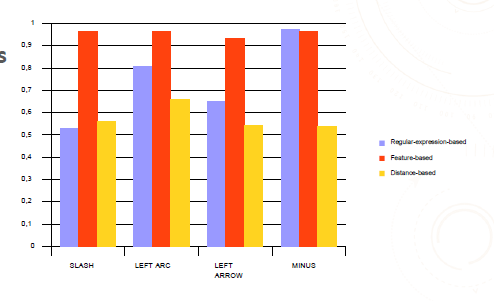
\includegraphics[scale=0.5]{img/gesture_recognition.png}
	\end{figure}\\
	Feature Based am genauesten, weil... ich glaub, dort die Referenzstrokes mit lernen, also während der Benutzung an den Nutzer angepasst werden
	
	\item Which touch events exist in typical toolkits? What information do the contain?\\
	Touch Start, Move, End, Cancel\\
	Enthalten Liste mit allen Touch Punkten seit die Geste gestartet wurde
	
	\item How can a multi-touch pinch gesture be detected on Android devices?\\
	ScaleGestureDetector mit Custom Listenr -> füge Detector an der View hinzu -> TouchEvent: verschicke Event an Detector -> Detector ruft listener, einmalig, wenn Geste identifiziert
	
	\item Discuss pros and cons of animated visual feedback!\\
	Änderung startet instantan -> fließender Übergang vom alten zum neuen Zustand durch Animation\\
	Pros: hilft die mentale Map aktuell zu halten\\
	Cons: benötigt Zeit, change blindness -> visuelle Veränderung vom Betrachter nicht wahrgenommen
	
	\item Sketch the main loop for animated feedback!
	\begin{enumerate}
		\item Process events
		\item Update Model
		\item render model
		\item Emit repaint Event, wenn mehr Updates notwendig sind
	\end{enumerate}
	
	\item Are there any studies regarding advantages and disadvantages of animation? ja
	
	\item What is the difference between timed animations and converging animations?
	Animation für eine konstante Zeitperiode; verschiedene Interpolationen (linear, slow-in, slow-out,..); einfacher Weg\\
	Converging: animiere bis Konvergenz erreicht ist; verschiedene Wege der Zustandübergangs (spring-mass, smooth and effizient zooming)
	
	\item What are easing functions good for?\\
	vermeiden das unnatürliche Verhalten einer linearen Animation (instantaner Start und Stopp)
	
	\item Explain animation via spring-mass systems (Masse Feder System)!\\
	Konvergierende Animation -> Zustand = Punktmassemit Pos. p, Beschleunigung a, und Geschwindigkeit v\\
	Übergang: Unterschied zw. Zuständen erzeugt Kraft; Kraft abhängig von der a der Punkte Masse in Richtung des neuen Zustandes -> a führt zu Bewegung\\
	Beende Animation, wenn Energie klein genug (und nicht am Ende des Weges); beachte: Feder schwingt ja quasi hin und her
	
	\item How can view navigation in ZUIs be enhanced with animation?\\
	smooth and efficient viewport animation (konvergierendes Verfahren)\\
	Idee: zoome heraus -> navigiere zum Punkt um zoome währenddessen wieder herein; mit Hilfe von Space Scale Diagram\\
	effizient = kürzester Pfad; smooth = keine wahrnehmbaren Unterbrechungen
	
	\item Contrast interactive lenses against regular interaction, discuss pros and cons?\\
	Lenses: leichtgewichtig; fokussieren temporäre Effekte\\
	regulär: schwergewichtig; haben globalen permanenten Effekt\\
	
	\item Give a definition of interactive lenses!\\
	Lens = Selection + alternative Representation + zusätzliches visuelles Feedback
	
	\item Sketch the conceptual model of lenses and the involved components!\\
	Input data: Selektion von Pixeln, Geometrien oder zugrundeliegenden Daten \\
	Data processing: Lens Funktion -> verarbeite Input für Linseneffekt; je nach Selektion nur Teilmenge der Verarbeitungsschritte notwendig; kleine Selektion => advanced Operations mgl\\\\
	-> 3 Linseneffekte: Veränderung; Ausblendung und Anreicherung
	Result output: Join -> führe Linseneffekt mit Hintergrund zusammen, auf dem Level von Pixeln, Geometrien oder underlying data
	
	\item How can lenses be interacted with?
	\begin{itemize}
		\item Positionierung mittels Maus und Parameterveränderung durch GUI (klassisch)
		\item Touch: bsp: zoom der Linse wie aufm Handy halt.. :D
		\item fühlbare/greifbare Interaktion: Bsp: Kunststoffring auf Tabletop als Linse -> von Software erkannt und platziert an Rings Position die Linse
		\item gaze-based: Interaktion mittels der Augenbewegungen
	\end{itemize}
	
	\item What is interaction syntax and why is it important?\\
	Menge von legalen Eingabesequenzen verbunden mit den Aktionen, die als Ergebnis auf die Eingabe aktiviert werden\\
	Wichtig für komplexe Interaktion -> erfordert viel Planung wie die Interaktion dem Nutzer gezeigt werden kann
	
	\item How can interaction syntax be specified? Discuss benefits and problems!\\
	\begin{itemize}
		\item Implizit durch Listener Logik -> führt zu Spaghetti Code
		\item Event Diagramme -> Pointer Positionen als Trajektorie + annotierte Events und Zustandsdarstellung entlang der Trajektorie -> sinnvoll für einfache Aufgaben, aber limitiert
		\item Interaction State Machines: sollte klar sein.. mit Hilfe von State Charts halt.. siehe SWT VL
	\end{itemize}
	
	\item Sketch a basic interaction using a state machine with guards!\\
	\begin{figure}[!h]
		\centering
		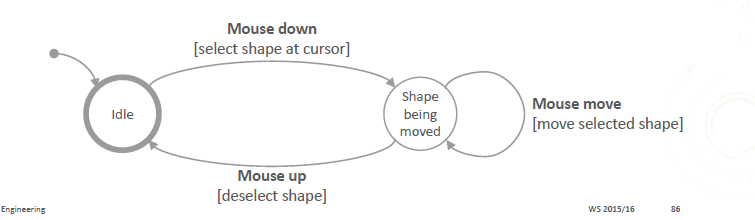
\includegraphics[scale=0.5]{img/state_interaction.png}
	\end{figure}
	
\end{itemize}